\section{The Relative ADP Framework}\label{Relative ADP Processors}

Now we present processors for our novel
relative ADP framework.
An \emph{ADP processor}\linebreak $\Proc$ has the form
$\Proc(\C{P},\C{P}^{=}) = \{(\C{P}_1,\C{P}^{=}_1), \ldots,
(\C{P}_n,\C{P}^{=}_n)\}$,  
where $\C{P}, \C{P}_1, \ldots, \C{P}_n,\linebreak \C{P}_1^{=}, \ldots, \C{P}_n^{=}$ are sets of ADPs. 
 $\Proc$ is \emph{sound} if $(\C{P},\C{P}^{=})$ is SN whenever 
$(\C{P}_i,\C{P}^{=}_i)$ is SN for all $1 \leq i \leq n$. 
It is \emph{complete} if
$(\C{P}_i,\C{P}^{=}_i)$ is SN for all 
$1 \leq i \leq n$ whenever $(\C{P},\C{P}^{=})$ is SN.
To prove relative termination of $\R/\R^=$, we start with the canonical ADP problem $(\ADPairMain{\R},\ADPairBase{\R^{=}})$
and apply sound 
(and preferably complete) ADP processors until all sub-problems are  transformed to the empty set.

In \Cref{Derelatifying Processors}, we
present two processors to remove (base) ADPs, and
in \Cref{Relative Dependency Graph Processor,Relative Reduction Pair Processor}, we adapt the main processors of the classical DP framework from \Cref{Dependency Pairs for Ordinary Term Rewriting}
to the relative setting.
As mentioned,  the soundness and completeness proofs for our processors and the chain criterion (\Cref{theorem:relative-chain-crit})
can be found in \Cref{Appendix}.

\subsection{Derelatifying Processors}\label{Derelatifying Processors}

The following two \emph{derelatifying} processors can be used to switch from ADPs to ordinary DPs,
similar to \Cref{theorem:main-relative-rewrite-corollary-yamada-1,theorem:main-relative-rewrite-corollary-yamada-2}.
We extend $\flat$ to ADPs and sets of ADPs $\SSS$
%JG $\Phi$ was used to denote sets of positions, whereas we use capital caligraphic
%letters for sets of (A)DPs.
by defining $\flat(\ell  \to r) = \ell \to \flat(r)$
and $\flat(\SSS) = \{\ell  \to \flat(r) \mid \ell \to r \in \SSS\}$.

If the ADPs in $\C{P}^{=}$ contain no annotations anymore,
then it suffices to use ordinary DPs.
The corresponding set of DPs for a set of ADPs $\C{P}$ is defined as 
$\DP{\C{P}} = \{\ell^\# \to t^\# \mid \ell \to r \in \C{P}, t \trianglelefteq_{\#} r\}$.

\begin{restatable}[Derelatifying Processor (1)]{theorem}{DerelProcOne}\label{theorem:derel-proc-1}
     Let $(\C{P}, \C{P}^{=})$ be an ADP problem such that $\flat(\C{P}^{=}) = \C{P}^{=}$.    
     Then $\Proc_{\mathtt{DRP1}}(\C{P}, \C{P}^{=}) = \emptyset$ is sound and complete
     iff the ordinary DP problem
     $(\DP{\C{P}}, \flat(\C{P} \cup \C{P}^{=}))$ \pagebreak[2] is SN.
\end{restatable}

Furthermore,  similar to \Cref{theorem:main-relative-rewrite-corollary-yamada-2},
we can always move ADPs from $\C{P}^{=}$ to $\C{P}$,
but such a processor is only sound and not complete.
However, it may help to satisfy 
the requirements of \Cref{theorem:derel-proc-1} by moving ADPs with 
annotations from $\C{P}^{=}$ to $\C{P}$ such that
the ordinary DP framework can be used  afterwards.

\begin{restatable}[Derelatifying Processor (2)]{theorem}{DerelProcTwo}\label{theorem:derel-proc-2}
    Let $(\C{P}, \C{P}^{=})$ be an ADP problem, and let $\C{P}^{=} = \C{P}^{=}_{a} \uplus \C{P}^{=}_{b}$.
    Then $\Proc_{\mathtt{DRP2}}(\C{P}, \C{P}^{=}) = \{(\C{P} \cup \mathtt{split}(\C{P}^{=}_{a}),
    \C{P}^{=}_{b})\}$ is sound.
    Here, $\mathtt{split}(\C{P}^{=}_{a}) = \{\ell \to \anno_{\pi}(r) \mid \ell \to r \in \C{P}^{=}_{a}, \pi \in \fun{pos}_{\SignatureD^\#}(r)\}$.    
\end{restatable}
\noindent
So if $\C{P}^{=}_{a}$ contains an ADP with two annotations, then we split it into two
ADPs, where each only contains
 a single annotation.

\begin{example}\label{terminatingRedexDuplCreate}
    There are also examples that are redex-creating and terminating, e.g., $\R_2 = \{ \ta \to \tb \}$ 
    and the base TRS $\R_2^{='} =
    \{ \tf(\ts(y)) \to \tc(\tf(y),\ta) \}$.
    Relative (and full) termination of this example can easily be
    shown by using
 the second derelatifying processor from \Cref{theorem:derel-proc-2} to
    replace the base ADP
    $\tf(\ts(y)) \to \tc(\tF(y),\tA)$ by the main ADPs $\tf(\ts(y)) \to \tc(\tF(y),\ta)$ and
    $\tf(\ts(y)) \to \tc(\tf(y),\tA)$. Then one can use the processor of
    \Cref{theorem:derel-proc-1} to switch to the ordinary DPs
$\tF(\ts(y)) \to \tF(y)$ and $\tF(\ts(y)) \to \tA$.
 \end{example}
  
\subsection{Relative Dependency Graph Processor}\label{Relative Dependency Graph Processor}

Next, we develop a dependency graph processor in the relative setting.
The definition of the dependency graph is analogous to the one in the standard setting and
thus, the same techniques can be used to over-approximate it automatically.

\begin{definition}[Relative Dependency Graph]\label{def:rel-dependency-graph}
    Let $(\C{P}, \C{P}^{=})$ be an ADP problem. 
    The $(\C{P}, \C{P}^{=})$-\defemph{dependency graph}
    has the nodes $\C{P} \cup \C{P}^{=}$ and there is an edge from
    $\ell_1 \to r_1$ to $\ell_2 \to r_2$ 
    if there exist substitutions $\sigma_1, \sigma_2$ and a term $t \trianglelefteq_{\#} r_1$ 
    such that $t^\# \sigma_1 \rightarrow_{\flat(\C{P} \cup \C{P}^{=})}^*
  \ell_2^\# \sigma_2$.
\end{definition}

So similar to the standard dependency graph,
there is an edge from an ADP $\ell_1 \to r_1$ to
$\ell_2 \to r_2$  if the rules of 
$\flat(\C{P} \cup \C{P}^{=})$ (without annotations) can reduce an instance of a
subterm $t$ of $r_1$ to an instance of $\ell_2$, if one only annotates
the roots of $t$ and $\ell_2$ (i.e., then the rules can only be applied below the root). 

\textcolor{white}{.}
\begin{wrapfigure}[5]{r}{0.42\textwidth}
            \scriptsize
        \vspace*{-1cm}
     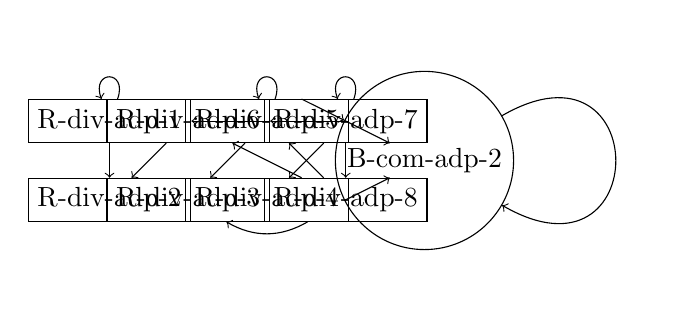
\begin{tikzpicture}
            \node[shape=rectangle,draw=black!100] (A) at (0,1) {\eqref{R-div-adp-1}};
            \node[shape=rectangle,draw=black!100] (B) at (0,0) {\eqref{R-div-adp-2}};
            \node[shape=rectangle,draw=black!100] (C) at (1,0) {\eqref{R-div-adp-3}};
            \node[shape=rectangle,draw=black!100] (D) at (2,0) {\eqref{R-div-adp-4}};
            \node[shape=rectangle,draw=black!100] (E) at (2,1) {\eqref{R-div-adp-5}};
            \node[shape=rectangle,draw=black!100] (F) at (1,1) {\eqref{R-div-adp-6}};
            \node[shape=rectangle,draw=black!100] (G) at (3,1) {\eqref{R-div-adp-7}};
            \node[shape=rectangle,draw=black!100] (H) at (3,0) {\eqref{R-div-adp-8}};
            \node[shape=circle,draw=black!100] (I) at (4,0.5) {\eqref{B-com-adp-2}};
        
            \path [->,in=110,out=70,looseness=5] (A) edge (A);
            \path [->] (A) edge (B);
            \path [->] (F) edge (A);
            \path [->] (F) edge (B);
            \path [->,in=110,out=70,looseness=5] (E) edge (E);
            \path [->] (E) edge (C);
            \path [->] (E) edge (F);
            \path [->,in=110,out=70,looseness=5] (G) edge (G);
            \path [->] (G) edge (D);
            \path [->] (G) edge (H);
            \path [->] (G) edge (I);
            \path [->,in=330,out=210,looseness=1] (H) edge (C);
            \path [->] (H) edge (E);
            \path [->] (H) edge (F);
            \path [->,in=330,out=30,looseness=5] (I) edge (I);
            \path [->] (I) edge (G);
            \path [->] (I) edge (H);
        \end{tikzpicture}
  \end{wrapfigure}

\vspace*{-.8cm}
\begin{example}\label{ex:rel-dependency-graph}
    The dependency graph for the ADP problem $(\ADPairMain{\R_{\tdivl}},
    \ADPairBase{\R^{=}_{\tset 2}})$
    from \Cref{ADP-Divl} is shown on the right. 
    Here, nodes from $\ADPairMain{\R_{\tdivl}}$ are denoted by rectangles and the
    node from $\ADPairBase{\R^{=}_{\tset 2}}$ is a circle.
\end{example}

To detect possible ordinary infinite rewrite sequences as in \Cref{example:ordinary-infinite},
we again have to regard SCCs of the dependency graph,
where we only need to consider SCCs that contain a node from $\C{P}$,
because otherwise, all steps in the SCC are relative.
However, in the relative ADP framework,
non-termination can also be due to chains representing redex-creating sequences.
Here,
it does not suffice to
look at SCCs.
Thus, the relative dependency graph processor differs substantially from the corresponding
processor for ordinary rewriting (and also from the corresponding processor for the
probabilistic ADP framework in \cite{FLOPS2024}). 

\begin{example}[Dependency Graph for Redex-Creating TRSs]\label{ex:DepGraphRedexCreating}
    For $\R_2$ and $\R_2^=$ from \Cref{example:redex-creating},
    the dependency graph for  $(\ADPairMain{\R_2}, \ADPairBase{\R_2^{=}})$ from
    \Cref{ex:ADPs-for-redex-creation-1} can be \pagebreak[2] seen on the

    \noindent
    \begin{minipage}[t]{9cm}
        right.
        Here, we cannot regard the SCC $\{\tf \to \tc(\tF,\tA)\}$ separately,
        as we need the rule  $\ta \to \tb$ from $\ADPairMain{\R_2}$ \linebreak
    \end{minipage}
    \hspace*{0.05cm}
    \begin{minipage}[t]{2.5cm}
        \begin{center}
            \scriptsize
            \vspace*{-0.4cm}
            \begin{tikzpicture}
                \node[shape=rectangle,draw=black!100] (A) at (0,0) {$\ta \to \tb$};
                \node[shape=rectangle,draw=black!100] (B) at (2,0) {$\tf \to \tc(\tF,\tA)$};
            
                \path [->,in=110,out=70,looseness=5] (B) edge (B);
                \path [->] (B) edge (A);
            \end{tikzpicture}
        \end{center}
    \end{minipage}

    \vspace*{-0.3cm}
    \noindent
    to reduce the created redex.
    To find the ADPs that can reduce the created redexes,
    we have to regard the outgoing paths
    from the SCCs of $\C{P}^=$  to ADPs of $\C{P}$. 
\end{example}

The structure that we are looking for in the redex-creating case is 
 a path from an SCC to a node from $\C{P}$
 (i.e., a form of a \emph{lasso}),
which is \emph{minimal} in the sense that if we reach a node from $\C{P}$, then we stop
and do not move further along the edges of the graph.
Moreover, the SCC needs to contain an ADP with more than one annotated symbol, as otherwise the
generation of the infinitely many
$\C{P}$-redexes would not be possible.
Here, it suffices to look at SCCs in the graph restricted to only $\C{P}^{=}$-nodes (i.e.,
to SCCs in the $(\flat(\C{P}),\C{P}^{=})$-dependency graph).
The reason is that
if the SCC contains a node from $\C{P}$, then as mentioned above,
we have to prove anyway
that the SCC does not give rise to infinite chains.


\begin{definition}[$\mathtt{SCC}^{(\C{P},\C{P}^{=})}_{\C{P}'}$, $\mathtt{Lasso}$]\label{def:lasso}
    Let $(\C{P},\C{P}^{=})$ be an ADP problem.
    For any $\C{P}' \subseteq \C{P} \cup \C{P}^{=}$,
    let $\mathtt{SCC}^{(\C{P},\C{P}^{=})}_{\C{P}'}$ denote 
    the set of all SCCs of the
    $(\C{P},\C{P}^{=})$-dependency graph that contain an ADP from
    $\C{P}'$. Moreover, let  $\C{P}^{=}_{>1} \subseteq \C{P}^{=}$ denote the set of all
    ADPs from $\C{P}^{=}$ with
    more than one annotation.
    Then the set of all \defemph{minimal lassos} is defined as
    $\mathtt{Lasso} = \{\QQ \cup \{n_1, \ldots, n_k\} \mid \QQ \in
    \mathtt{SCC}^{(\flat(\C{P}),\C{P}^{=})}_{\C{P}^{=}_{>1}}, \; n_1,\ldots,n_k$ is a path such that $n_1 \in \QQ, \; n_k \in \C{P}, \text{ and } n_i \not\in \C{P} \text{ for all } 1 \leq i \leq k-1\}$.
\end{definition}

We remove the annotations of ADPs which do not have to be considered anymore\linebreak for
$\mathbf{p}$-steps due to the dependency graph, 
but we keep the ADPs for possible $\mathbf{r}$-steps and thus, consider
them as relative (base) ADPs.

\begin{restatable}[Dep.\ Graph Processor]{theorem}{RelativeDepGraphProc}\label{theorem:rel-DGP}
    Let $(\C{P},\C{P}^{=})$ be an ADP problem.
    Then

    \vspace*{-.4cm}
    
    {\small\begin{align*}
        \Proc_{\mathtt{DG}}(\C{P},\C{P}^{=}) & =
        \{ (\,\C{P} \cap \QQ, \;
        (\C{P}^= \cap \QQ)\cup        \flat( \,(\C{P} \cup \C{P}^{=}) \setminus \QQ \,)\,
           )
        \mid \QQ
        \in \mathtt{SCC}_{\C{P}}^{(\C{P}, \C{P}^{=})} \cup \mathtt{Lasso}\} \! 
    \end{align*}
    }

    \vspace*{-.1cm}

    \noindent
    is sound and complete.   
\end{restatable}

\begin{example}\label{ex:DivlDepGraph}
    For $(\ADPairMain{\R_{\tdivl}}, \ADPairBase{\R^{=}_{\tset 2}})$ from
    \Cref{ex:rel-dependency-graph} we have three SCCs 
    $\{\eqref{R-div-adp-1}\}$, $\{\eqref{R-div-adp-5}\}$, 
    and $\{\eqref{R-div-adp-7},\eqref{B-com-adp-2}\}$ containing nodes from $\ADPairMain{\R_{\tdivl}}$.
    The set $\{\eqref{B-com-adp-2}\}$ is the only
    SCC of $(\flat(\ADPairMain{\R_{\tdivl}}), \ADPairBase{\R^{=}_{\tset 2}})$ and there
    are paths from that SCC to the ADPs $\eqref{R-div-adp-7}$ and
    $\eqref{R-div-adp-8}$ of $\C{P}$. However, they are not in
    $\mathtt{Lasso}$, because the SCC $\{\eqref{B-com-adp-2}\}$ does not contain an ADP with more than one
    annotation.
    Hence, we result in the three new ADP problems 
    $(\{\eqref{R-div-adp-1}\} \cup \flat(\ADPairMain{\R_{\tdivl}} \setminus \{\eqref{R-div-adp-1}\}), \{\flat(\ref{B-com-adp-2})\})$,
    $(\{\eqref{R-div-adp-5}\} \cup \flat(\ADPairMain{\R_{\tdivl}} \setminus \{\eqref{R-div-adp-5}\}), \{\flat(\ref{B-com-adp-2})\})$,
    and 
    $(\{\eqref{R-div-adp-7}\} \cup \flat(\ADPairMain{\R_{\tdivl}} \setminus \{\eqref{R-div-adp-7}\}),\{(\ref{B-com-adp-2})\})$.
    For the first two of these new ADP problems, 
    we can use the derelatifying processor of \Cref{theorem:derel-proc-1} and prove SN via ordinary DPs, since their base
    ADP $\flat(\ref{B-com-adp-2})$ does not contain any annotated symbols anymore.
\end{example}

The dependency graph processor in combination with the derelatifying processors of \Cref{theorem:derel-proc-1,theorem:derel-proc-2}
already subsumes the techniques of
\Cref{theorem:main-relative-rewrite-corollary-yamada-1,theorem:main-relative-rewrite-corollary-yamada-2}.
The reason is that if $\R$ dominates $\R^{=}$, then there is no edge from an ADP of $\ADPairBase{\R^{=}}$ to
any ADP of $\ADPairMain{\R}$ in the $(\ADPairMain{\R}, \ADPairBase{\R^{=}})$-dependency
graph. Hence, there are no minimal lassos and the
dependency graph processor just creates ADP problems from the SCCs of $\ADPairMain{\R}$
where the base ADPs do not have any annotations anymore. Then \Cref{theorem:derel-proc-1}
allows us to switch to ordinary DPs.
For example, if we consider $\R^{=}_{\tset}$ instead of $\R^{=}_{\tset 2}$, then the
dependency graph processor \pagebreak[2]  only yields the two subproblems for the SCCs 
$\{\eqref{R-div-adp-1}\}$ and $\{\eqref{R-div-adp-5}\}$, 
where the base ADPs do not\linebreak contain any annotations anymore.
Then, we can move to ordinary
DPs via \Cref{theorem:derel-proc-1}.

Compared to
\Cref{theorem:main-relative-rewrite-corollary-yamada-1,theorem:main-relative-rewrite-corollary-yamada-2},
the dependency graph allows for more precise
over-approximations than just ``dominance'' in order
to detect when the base ADPs do not depend on 
the main ADPs.  Moreover,
the derelatifying processors of \Cref{theorem:derel-proc-1,theorem:derel-proc-2}
allow us to switch to  the ordinary DP framework also for subproblems which result 
from the application of other processors of our relative ADP framework.
In other words, \Cref{theorem:derel-proc-1,theorem:derel-proc-2} allow us to apply this
switch in a modular way, even if their prerequisites
do not hold for the initial canonical ADP problem (i.e., even if the prerequisites of \Cref{theorem:main-relative-rewrite-corollary-yamada-1,theorem:main-relative-rewrite-corollary-yamada-2}
do not hold for the whole TRSs).


\subsection{Relative Reduction Pair Processor}\label{Relative Reduction Pair Processor}

Next, we adapt the reduction pair processor to ADPs for relative rewriting.
While the reduction pair processor for ADPs in the probabilistic setting
\cite{FLOPS2024} was restricted to polynomial interpretations,
we now allow arbitrary
reduction pairs
using a similar idea as in 
the reduction pair processor from \cite{noschinski2013analyzing} for complexity analysis
via dependency tuples.

To find out which ADPs cannot be used for infinitely many $\mathbf{p}$-steps,
the idea is not to compare the annotated left-hand side with the
whole right-hand side, but just with the set of its annotated subterms.
To combine these subterms in the case of
ADPs with two or no annotated symbols, we extend the signature by two fresh \emph{compound} symbols
$\Com{0}$ and $\Com{2}$ of arity $0$ and $2$, respectively.
Similar to \cite{noschinski2013analyzing},
we have to use $\Com{}$\emph{-monotonic} and $\Com{}$\emph{-invariant} reduction pairs.

\begin{definition}[$\Com{}$-Monotonic, $\Com{}$-Invariant]\label{def:poly-interpretation-for-depset}
    For $r \in \TSet{\SignatureADC}{\VSet}$, we define
    $\subA(r) = \Com{0}$ if $r$ does not contain any annotation,
    $\subA(r) = t^\#$ if $t \trianglelefteq_{\#} r$ and $r$ only contains one annotated symbol,
    and $\subA(r) = \Com{2}(r_1^\#, r_2^\#)$ if $r_1 \trianglelefteq_{\#}^{\pi_1} r$,
    $r_2 \trianglelefteq_{\#}^{\pi_2} r$, 
    and $\pi_1 <_{lex} \pi_2$ where $<_{lex}$ is the (total)
    lexicographic order on positions.

    A reduction pair $(\succsim, \succ)$ is called \defemph{$\Com{}$-monotonic}
    if $\Com{2}(s_1, t) \succ
    \Com{2}(s_2, t)$ and $\Com{2}(t, s_1) \succ
    \Com{2}(t, s_2)$ for all $s_1,s_2,t \in \TSet{\SignatureADC}{\VSet}$ with $s_1 \succ s_2$.
    Moreover, it is  \defemph{$\Com{}$-invariant}
    if $\Com{2}(x,y) \sim \Com{2}(y,x)$ and
    $\Com{2}(x,\Com{2}(y,z)) \sim 
    \Com{2}(\Com{2}(x,y),z)$
    for ${\sim} = {\succsim} \cap {\precsim}$. 
\end{definition}
So for example, reduction pairs based on polynomial interpretations are
$\Com{}$-monotonic and $\Com{}$-invariant if $\Com{2}(x,y)$ is interpreted by $x + y$.

For an ADP problem $(\C{P},\C{P}^{=})$, 
now the reduction pair processor has to orient the non-annotated rules $\flat(\C{P} \cup
\C{P}^{=})$ weakly and for all ADPs $\ell \to r$,
it compares the annotated left-hand side  $\ell^\#$ with
$\subA(r)$. In strictly decreasing ADPs, one can then remove all annotations and consider
them as relative (base) ADPs again.

\begin{restatable}[Reduction Pair Processor]{theorem}{RelRPP}\label{thm:RelRPP}
    Let $(\C{P},\C{P}^{=})$ be an ADP problem and let
    $(\succsim, \succ)$ be a $\Com{}$-monotonic and $\Com{}$-invariant reduction pair
    such that $\flat(\C{P} \cup \C{P}^{=})\linebreak \subseteq {\succsim}$ and
    $\ell^\# \succsim \subA(r)$ for all $\ell \to r \in \C{P} \cup \C{P}^{=}$.
    Moreover, let $\PP_{\succ} \subseteq \C{P} \cup \C{P}^{=}$ 
    such that\linebreak $\ell^\# \succ \subA(r)$ for all $\ell \to r \in \PP_{\succ}$. 
    Then $\Proc_{\mathtt{RPP}}(\C{P},\C{P}^{=}) = \{(\C{P} \setminus \PP_{\succ}, (\C{P}^{=} \setminus \PP_{\succ}) \cup
    \flat(\PP_{\succ}))\}$ is sound and complete.
\end{restatable}

\begin{example}\label{example:rel-RPP}
    For the remaining ADP problem
    $(\{\eqref{R-div-adp-7}\} \cup \flat(\ADPairMain{\R_{\tdivl}} \setminus \{\eqref{R-div-adp-7}\}),\{(\ref{B-com-adp-2})\})$ 
    from \Cref{ex:DivlDepGraph}, we can apply the reduction pair processor
    using the polynomial interpretation from the end of \Cref{Dependency Pairs for Ordinary Term Rewriting} which maps 
    $\O$ to $0$, $\ts(x)$ to $x + 1$,
    $\tcons(y,\xs)$ to $\xs + 1$, $\tDL(x,\xs)$ to $\xs$,
    and all other symbols to their first arguments. 
    Then, $\eqref{R-div-adp-7}$ is oriented strictly (i.e., it is in
    $\PP_{\succ}$) and $\eqref{B-com-adp-2}$ is oriented weakly.
    Hence, we remove the annotation from $\eqref{R-div-adp-7}$ and move it to the base
    ADPs.
    Now there is no SCC with a main ADP anymore in the
    dependency graph, and thus the dependency graph processor 
    returns $\emptyset$.
    This proves SN for $(\ADPairMain{\R_{\tdivl}}, \ADPairBase{\R^{=}_{\tset 2}})$, hence
    $\R_{\tdivl} / \R^{=}_{\tset 2}$ is also SN.
\end{example}

\begin{example}\label{ex:RPPCreating}
    Regard the ADPs
    $\ta \to \tb$  and $\tf \to \tc(\tF,\tA)$ for
    the redex-creating  \Cref{example:redex-creating} again.
    When using  a polynomial interpretation  $\mathrm{Pol}$ that maps $\Com{0}$ to $0$ and
    $\Com{2}(x,y)$ to $x + y$, then for the reduction pair processor 
    one has to satisfy $\mathrm{Pol}(\tA) \geq 0$ and
    $\mathrm{Pol}(\tF) \geq \mathrm{Pol}(\tF) + \mathrm{Pol}(\tA)$, i.e.,
    one cannot
    make any of the ADPs strictly decreasing.

    In contrast, for the variant
    with the terminating base rule  $\tf(\ts(y)) \to \tc(\tf(y),\ta)$ from \Cref{terminatingRedexDuplCreate},
    we have the ADPs $\ta \to \tb$  and $\tf(\ts(y)) \to \tc(\tF(y),\tA)$. 
    Here, the second constraint is  $\mathrm{Pol}(\tF(\ts(y))) \geq
    \mathrm{Pol}(\tF(y)) + \mathrm{Pol}(\tA)$. To make 
    one of the ADPs strictly decreasing,
    one can set
    $\mathrm{Pol}(\tF(x)) = x$, $\mathrm{Pol}(\ts(x)) = x+1$, and
    $\mathrm{Pol}(\tA) = 1$ or $\mathrm{Pol}(\tA) = 0$.
    Then the reduction pair processor
    removes the annotations from the strictly decreasing ADP and 
     the dependency graph processor  proves SN.
\end{example}
